\chapter{Introduction}
\label{chp:intro}


%%%%%%%%%%%%%%%%%%%%%%%%%%%%%%%%%%%%%%%%%%%%%%%%%%%%%%%%%%%%%%%%%%%%%%%
\section{Background}

Here you write your amazing text.\footnote{You include footnotes like this.} With examples of two types of citations. Some citations happen in parenthesis, for example \parencite[215]{Abma2000} , whilst others are cited in text, such as \textcite[4]{Ancora2012} said that sometimes you want to cite multiple authors at one point, which you do like this \parencite{Czarniawska2000, Weick1995}.

In a later article \parencite[410-413]{Weick2005} the properties are called ``distinctive features'' of sensemaking. 
Note how quotations marks look in TeX, especially the opening ones that can be found near Z on your keyboard and the closing ones that are \emph{TWO} individual ones found near your Return key (and now you know how to make things italics with the emph-command).

\subsection{Next level heading}

Yet more boring text to write and read. You have to write 100-120 pages, but no more than 140. Anything under 100 pages of text is likely too short.

\subsubsection{Third level heading}
At a push you might need even another level down, but think carefully about third level subheadings.

\subsubsection{Another third level heading}
Remember that if you go down a level, the level must always have at least one partner on the same level, otherwise why did you need to go down a level?

\subsection{How to do tables}

Another thing you might want to do is to include a table. This is the only really difficult thing in LaTeX and I propose that you use \url{https://www.tablesgenerator.com/latex_tables} and making your tables in excel, save them as CSV-files and then open them on that site and generate the code there, copy and paste it back in your text. Remember to use the caption and booktabs options for nice looking tables.\footnote{And now you also know how to insert URLs in the text.} 

%%% One can add the option [H] to the table generated, which ensures the table is placed always below the text above. If you leave the option open, then the software decides where to place it best. Usually the default is good enough.
%Possible values are: 
%h (here) - same location
%t (top) - top of page
%b (bottom) - bottom of page
%p (page) - on an extra page
%! (override) - will force the specified location when written behind a value as in [h!]

\begin{table}[h]
\centering
\begin{tabular}{@{}lll@{}}
\toprule
\textbf{SECI} & Tacit           & Explicit        \\ \midrule
Tacit         & Socialization   & Externalization \\
Explicit      & Internalization & Combination     \\ \bottomrule
\end{tabular}
\caption{Nonaka's SECI-model}
\label{tab:seci}
\end{table}

Here you simply continue writing your text. The labels command after sections, tables, or figures and so on can be used for cross-references, like Table \ref{tab:seci} shows the knowledge conversion processes.

\subsection{How to make lists}

You may for instance think that you need to make a list. Such a list can be either bulleted.

\begin{itemize}
	\item apples
	\item oranges
	\item pears
\end{itemize}

Alternatively a list may be numbered like the one here:

\begin{enumerate}
	\item dogs
	\item cats
	\item hamsters
\end{enumerate}

But remember that writing paragraphs are always better than writing lists, because paragraphs contain arguments with reasons, whilst lists only describe. Therefore please do not overuse the list function.

\subsection{How to include figures}

Make sure that you have the figure saved in a format that autoscales easily and in the appropriate folder called ``figs''. Then you include it with the following commands.

\begin{figure}[h]
  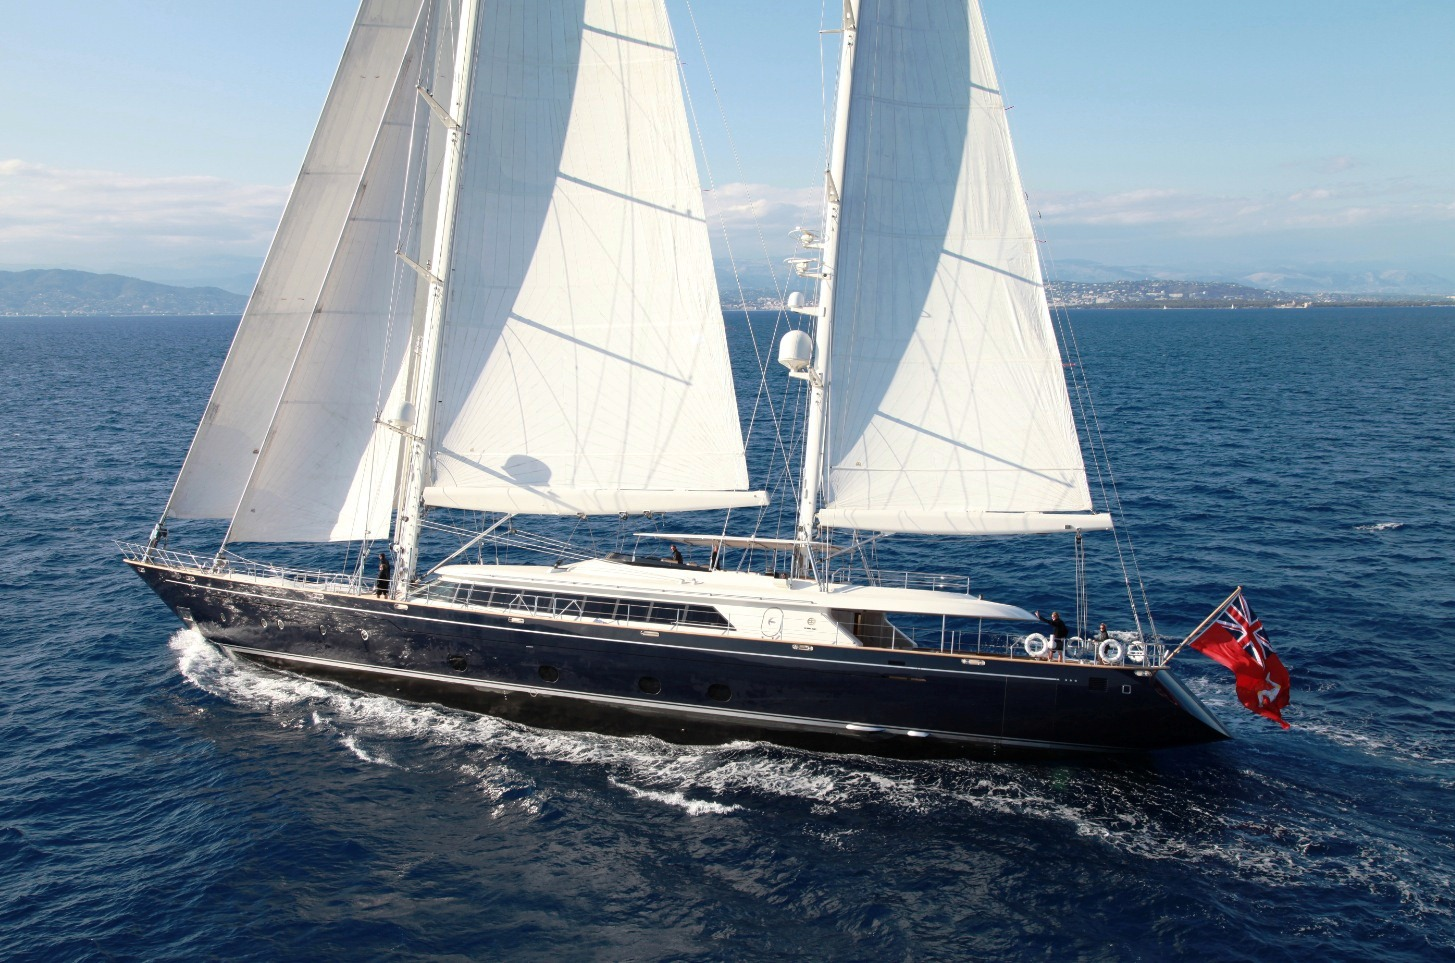
\includegraphics[width=\linewidth]{figs/boat.jpg}
  \caption{A boat.}
  \label{fig:boat1}
\end{figure}

As you can see Figure \ref{fig:boat1} shows a boat.

\subsection{Conclusion}

This should be enough to get you started. You just write in the Chapter files with these few basic commands, you will see that the root-file will include the individual chapter files in the US-thesis wrapper.